
%\pgfplotstableread[col sep=comma]{../evaluation_translations/combined_smolsent_bleurt_scores_madlad.csv}\combinedSmolSentBLEURT

\newcommand\resultplot[6]
{\pgfplotsset{
    % initialize Set1-5:
    cycle list/Set1-5,
    % combine it with 'mark list*':
    cycle multiindex* list={
        mark list*\nextlist
        Set1-5\nextlist
      },
  }
  \pgfplotstableread[col sep=comma]{#2}\accutable
  \pgfplotstableread[col sep=comma]{#3}\timetable

  \begin{minipage}{\textwidth}
    \begin{tikzpicture}
      \begin{axis}[
          name=timeax,
          xmajorgrids=true, ymajorgrids=true,
          xlabel={Noise}, ylabel={Accuracy},
          xtick=data,
          xticklabels={0, 5, 10, 15, 20, 25},
          %log number format basis/.code 2 args={$\pgfmathparse{#1^(#2)}\mathsf{\pgfmathprintnumber{\pgfmathresult}}$},
          %yticklabels=={$\pgfmathprintnumber[precision=0]{\tick}$},
          %syticklabels={0.4, 0.3, 0.5, 0.6, 0.7, 0.8, 0.9, 1.0},
          %legend style={at={(0.5,-0.16)}, anchor=north, legend columns=2, font=\footnotesize, legend cell align={left}},
          width=\textwidth*0.45,
          height=\textwidth*0.45,
        ]
        \pgfplotsforeachungrouped \i in {0,...,#4} {
            \addplot table[x expr=\coordindex, y index=\i]
              {\accutable};
          }
      \end{axis}
      \begin{semilogyaxis}[
          at={(timeax.south east)},
          xshift=2cm,
          xmajorgrids=true, ymajorgrids=true,
          xlabel={Noise}, ylabel={Time (s)},
          xtick=data,
          xticklabels={0, 5, 10, 15, 20, 25},
          %log number format basis/.code 2 args={$\pgfmathparse{#5^(#6)}\mathsf{\pgfmathprintnumber{\pgfmathresult}}$},
          %yticklabels={0.1, 1, 10, 100, 1000},
          legend style={at={(-0.25,-0.25)}, anchor=north, legend columns=3, font=\footnotesize, legend cell align={left}},
          width=\textwidth*0.45,
          height=\textwidth*0.45,
        ]
        \pgfplotsforeachungrouped \i in {0,...,#4} {
            \addplot table[x expr=\coordindex, y index=\i]
              {\timetable};
          }
        \ifthenelse{\equal{#5}{true}}{
          %\legend{\textsc{Fugal}, \textsc{cuGAL-Mix}, \textsc{cuGAL-Mix} $\gamma=0.1$, \textsc{cuGAL-Mix} $\gamma=0.2$,\textsc{cuGAL-Mix-Greedy}, \textsc{cuGAL-Mix-Greedy} $\gamma=0.1$, \textsc{cuGAL-Mix-Greedy} $\gamma=0.2$,\textsc{cuGAL-Log}, \textsc{cuGAL-Log} $\gamma=0.1$, \textsc{cuGAL-Log} $\gamma=0.2$, \textsc{cuGAL-Log-Greedy}, \textsc{cuGAL-Log-Greedy} $\gamma=0.1$, \textsc{cuGAL-Log-Greedy} $\gamma=0.2$}
          \legend{#6}
        }{}
      \end{semilogyaxis}
    \end{tikzpicture}
    \captionof{figure}{Runtime and accuracy on #1 dataset}
    \label{fig:#1_res}
  \end{minipage}
}

\newcommand{\BLEURTresults}{
  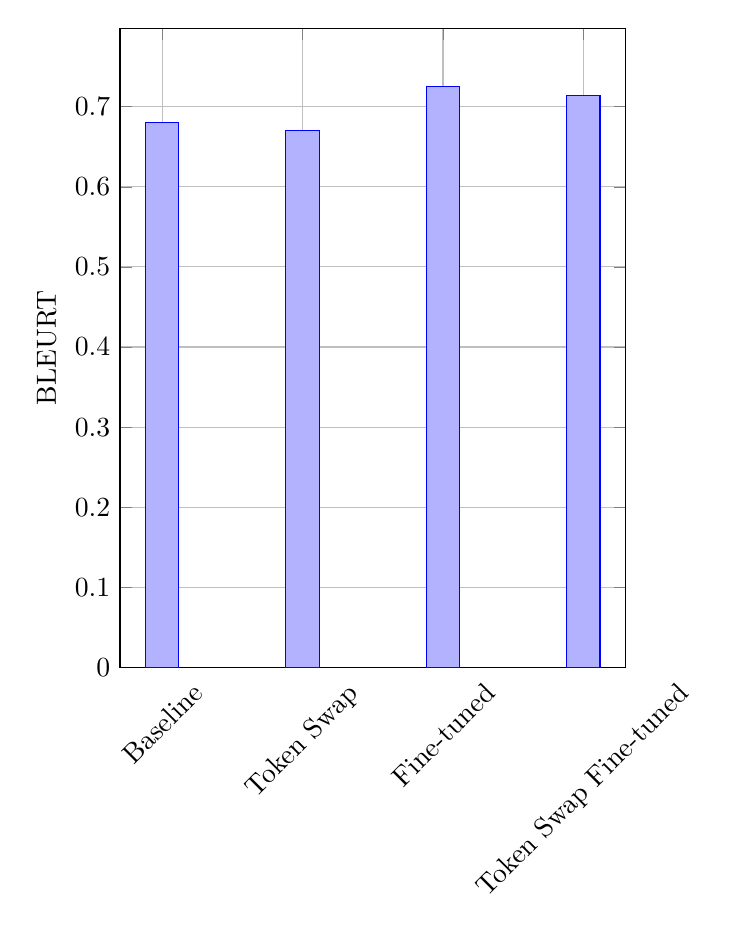
\begin{tikzpicture}
    \begin{axis}[
        ybar stacked,
        ymin=0,
        xtick=data,
        xticklabels={Baseline,Token Swap,Fine-tuned,Token Swap Fine-tuned},
        x tick label style={rotate=45},
        legend style={at={(0.5, -0.2)}, anchor=north, legend columns=-1},
        bar width=12pt,
        width=\textwidth*0.66,
        height=\textwidth*0.8,
        ylabel={BLEURT},
        ymajorgrids=true,
        xmajorgrids=true,
      ]
      \addplot coordinates {
          (0, 0.6806566989284822)
          (1, 0.6704189777374268)
          (2, 0.7254119131756925)
          (3, 0.7144110394620348)
        };
    \end{axis}
  \end{tikzpicture}
}

\newcommand{\BLEURTtokenreplacementviolin}{
  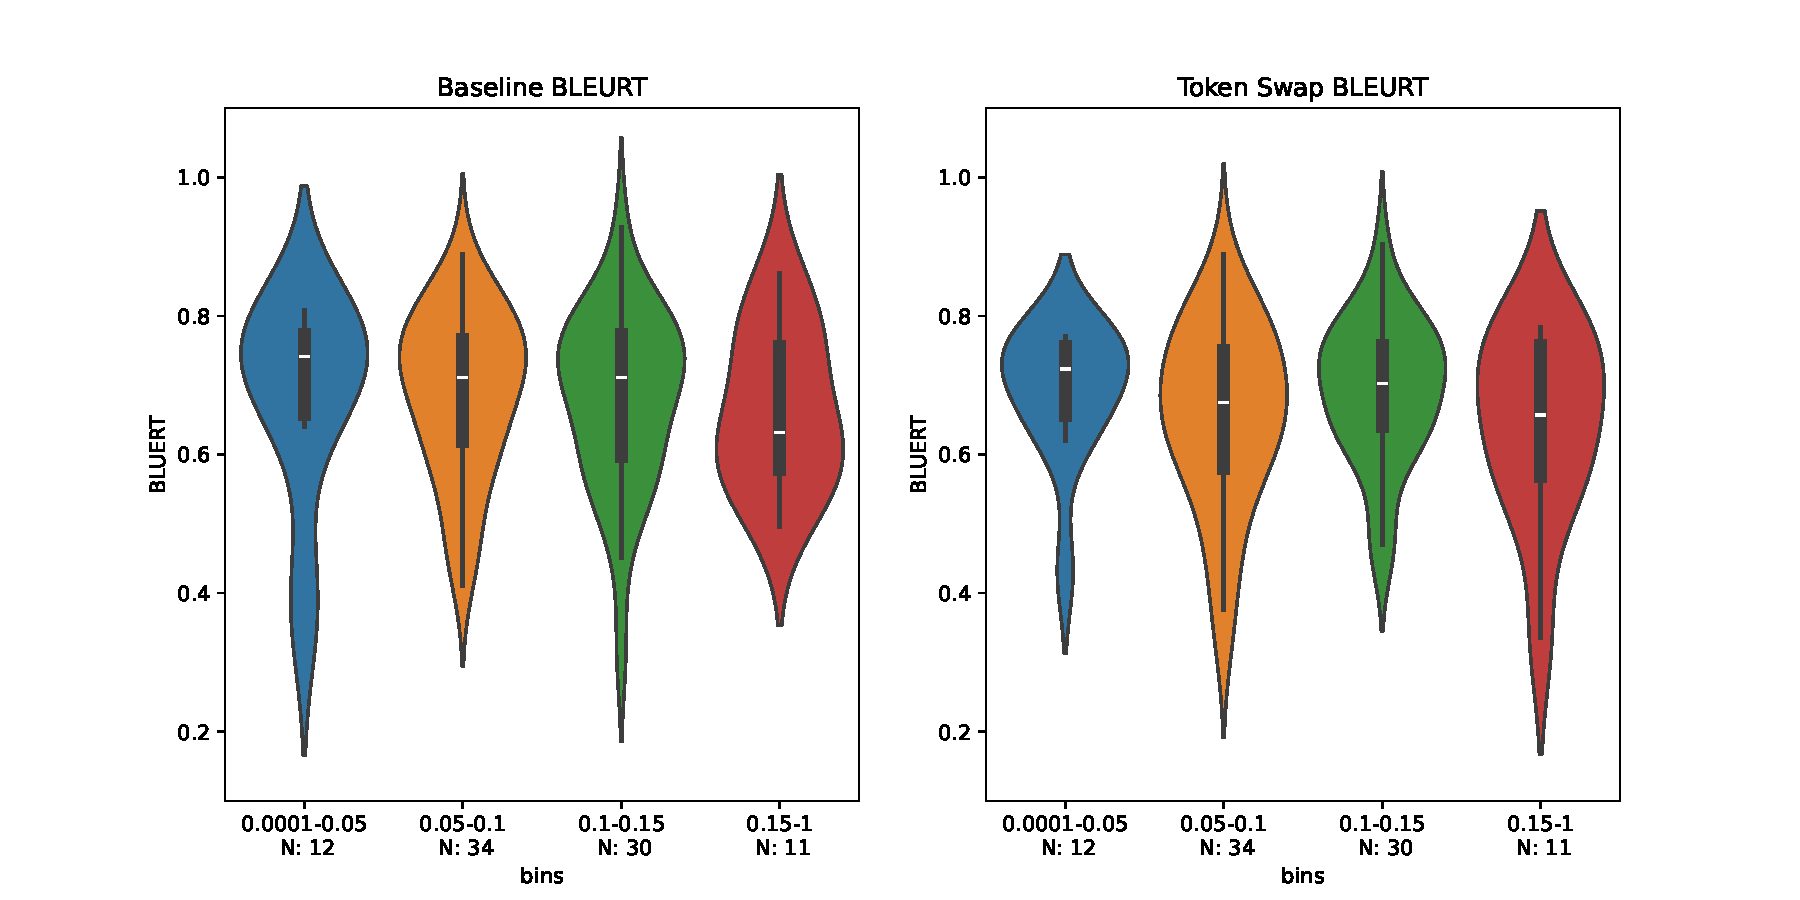
\includegraphics[width=\textwidth]{data_and_figs/TS_BLEURT_violin.pdf}
}

\newcommand{\tokenreplacementexample}{
  \def\arraystretch{1.3}%
  \begin{tabular}{ | p {0.25\textwidth} | p {0.25\textwidth} | p {0.25\textwidth} | p {0.15\textwidth} | }
    \hline
    \textbf{Source}                                                                                      & \textbf{Baseline}                                                                          & \textbf{Token Replacement}                                                                      & \textbf{$\Delta$ BLEURT} \\
    \hline
    Rohan was my sibling who always flew a kite at noon, even if it was cloudy.                          & The bridge is opened to the public at noon, and closed at midnight.                        & Rohan is my brother, and he flies kites at noon every day, even when the sky is dark.           & 0.449354                 \\
    \hline
    From 10 feet away you could tell the bottom of the boat was in rough shape.                          & It was very bad from 10 feet away.                                                         & The bottom was in poor condition and visible from a distance of 10 feet;                        & 0.246233                 \\
    \hline
    It includes a legend of a devil beast, a century-old family curse.                                   & It includes a legendary demon beast, a family curse that has lasted for hundreds of years. & He is the one who has been the master of the witchcraft for centuries.                          & -0.379743                \\
    \hline
    Bear in mind, constantly try to purchase silk plants, as they tend to appear like the genuine thing. & Remember, keep trying to buy silk plants because they look like real ones.                 & They are often used to make the plant's leaves and flowers look like they are actually flowers. & -0.291243                \\
    \hline
  \end{tabular}
}